\section{Research Method}

%   How can I assess the quality of my Methods section? To make a self-assessment of your Methods section, you can ask yourself the following questions.
%    * Have I really described my Methods in a way that is easy for readers to follow and which would enable them to replicate my work? Have I ensured that I have covered every step? Is my structure clear and complete?
%    * Have I been as concise as possible? Have I used references to previous works rather than repeating descriptions that readers could easily find elsewhere?
%    * Do the individual sentences in each paragraph contain too many, too few, or just the right manageable number of steps? Have I ensured that my sentences don’t sound like lists?
%    * Have I thought about the way readers prefer to receive information? (no ambiguity, no back referencing, everything in chronological order, headings, bullets)?
%    * Have I checked my grammar (infinitive, gerund, allow, thus etc.) with regard to how I outline how and why I made certain choices?
%    * Have I checked my journal’s guidelines on how to use numbers?
%    * Have I used tenses correctly? past simple (in the passive form to describe what I did), present simple (descriptions of established scientific fact)

This study performed a mapping study about the usage of Machine Learning techniques for code smells identification. SLRs are reviews organized and based on a clear search strategy, that ensures the rigor, completeness and reproducibility of the process, focusing on the identification, evaluation and interpretation of the available research that is relevant to a particular question~\citep{kitchenham2010systematic}.

In order to accomplish the SLR the following steps were taken: planning, defining research questions, searching databases, discussion of validity, data extraction, and synthesis of the results, those steps are in accordance to the typical steps taken for a SLR~\citep{keele2007guidelines}. The following subsections embrace each of those steps.

\subsection{Planning}

We developed a review protocol in order to ensure that the research is executed in a planned way and not driven by the researcher expectations according to the guidelines provided by Kitchenham et al.~\cite{kitchenham2015evidence}. In the protocol, the following items were addressed as part of the planning for the study: research objectives; research questions; search strategy; study selection, studies quality assessment; data extraction; and data synthesis and aggregation.

\subsection{Research Questions}

 This research focuses on the identification machine learning techniques for code smells identification and in order to accomplish that the following questions must be addressed: 

\begin{itemize}
    \item \textbf{RQ1: Which code smells are addressed by articles using machine learning techniques for code smells identification?}
    RQ1 focuses on the most studied code smells covered by the literature. It can help identify which code smells have not been explored in existing research and can be used as gaps for future works.
    \item \textbf{RQ2: Which machine learning techniques are used when identifying code smells?} 
    RQ2 aims in the identification of machine learning techniques  commonly used to identify code smells and it can list potential machine learning techniques that were not yet explored for this specific task.
    \item \textbf{RQ3: Which machine learning techniques are most used for each kind of code smell?}
    RQ3 is concerned with the relationship between the machine learning techniques and the code smells in research papers allowing the identification of which techniques are used for each of the code smells. It could also lead us to identify potential machine learning techniques that can be used for similar code smells but have not yet being used with this intent.
    \item \textbf{RQ4: Which machine learning techniques performs better for each code smell?}
    RQ4 compares the performance of different machine learning techniques for code smell detection. The answer to this question can help researchers define which machine learning techniques to use when studying different types of code smells.
\end{itemize}

\subsection{Search Strategy}

In order to find relevant articles to achieve the goals of this study, we conducted searches based on the recommendations by Kitchenham et al.~\cite{kitchenham2015evidence}. In the first step, we used personal experience to define the list of journals and conferences, summarized in table~\ref{tab:ManualSearchSources}, used to establish the quasi-gold standard. The digital libraries selected for automated searches were ACM, IEEE, Science Direct and Wiley.

was used in manual searches by two of the authors authors and 69 articles resulted of the .
in four digital libraries - ACM, IEEE, Science Direct and Wiley - for papers published up to 2016. The definition of the search string followed these steps based :
\begin{enumerate}
    \item{Derived major terms for machine learning and code smells from research questions.}
    \item{Broke major terms down into smaller terms.}
    \item{Identified alternative spellings or synonyms for the smaller terms.}
    \item{Checked the search terms in known relevant papers.}
    \item{Used Boolean operator OR to combine alternative spellings and synonyms. Used Boolean operator AND to link machine learning and code smells terms.}
\end{enumerate}

The following search string was then generated: "("code smell" OR "bad smell") AND ("learning" OR "data mining" OR "artificial intelligence" OR "pattern recognition" OR "case based reasoning" OR "decision tree" OR "regression tree" OR "classification tree" OR "neural net" OR "genetic programming" OR "genetic algorithm" OR "Bayesian belief network" OR "Bayesian net" OR "association rule" OR "support vector machine" OR "support vector regression")". 

This filter returned 1021 papers, distributed as shown in Figure \ref{fig:librariesImage}. The search string tries to filter papers that applies Machine Learning techniques for code smell identification problems.

\begin{figure}[hbt] 
	\caption{Distribution of papers by article}
	\label{fig:librariesImage}
	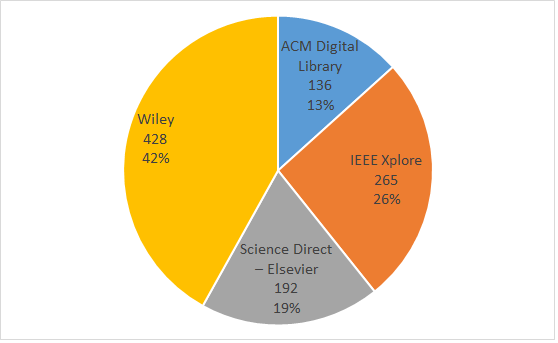
\includegraphics[width=0.95\textwidth]{imagens/librariesDistributionImage.png}
\end{figure}

After the filtering, 338 duplicated results were removed, resulting in 683 remaining results. Following to that publications which were not papers or proceedings papers which belonged to a Journal that is not related to Computational Fields were removed and, leaving 286 results left. The studies were then filtered by the publication title, removing any study which was not related to the usage of Machine Learning techniques for code smells identification, what left 155 results. This same criteria was applied when filtering by abstract, resulting in 53 papers left for classification. These steps were summarized in Figure \ref{fig:paperScreening}  Each step was peer reviewed by graduated students, the  results were compared and discussed to reach a consensus.

\begin{figure}[hbt] 
    \centering
    \caption{Paper screening process}
	\label{fig:paperScreening}
	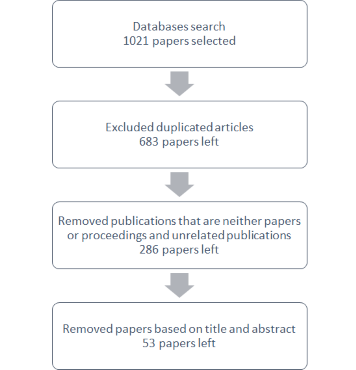
\includegraphics[]{imagens/paperScreening.png}
\end{figure}

The inclusion and exclusion criteria for those filters were defined as follows:

\noindent \textbf{Inclusion criteria:}
\begin{itemize}
    \item Articles describing the use of methods and that establish the relationship between machine learning and code smells.
    \item The studies publication type must be journals or conferences
\end{itemize}

\noindent \textbf{Exclusion criteria:}
\begin{itemize}
    \item Remove duplicates
    \item Remove studies where the code smells identification are done manually
    \item Remove non-empirical studies
\end{itemize}

\subsection{Quality assessment}

The main purpose of this study is to cover papers about the usage of Machine Learning Techniques for Code Smell identification. In order to try to avoid the non inclusion of relevant papers  precautions were taken. One of the cautions made was to include keywords, title, and abstract in the search, we also took the precaution of including synonyms and abbreviates.

Clear criteria for the exclusion and exclusion of the papers were also defined prior to the study. And each steps was registered so it could be evaluated by external parties. To assert the results of the study, peer reviews done by two graduated researchers were executed, compared and discussed in order to reach a consensus and avoid the perception of the researcher to influence the results. Criteria for classification was also selected from related works and explicit defined before the execution of the review.

The following questions were taken to improve the reliability of the work and avoid missing relevant papers:
\begin{itemize}
    \item \textbf{QA1}: Are the aims of the research defined explicitly?
    \item \textbf{QA2}: Is the context related to code smells?
    \item \textbf{QA3}: Are the used techniques exposed and related to Machine Learning?
    \item \textbf{QA4}: Is the experimental design appropriate and justifiable?
    \item \textbf{QA5}: Is the proposed estimation method comparable with other methods?
    \item \textbf{QA6}: Are the findings of study stated and supported by reporting results?
    \item \textbf{QA7}: Does the study add value to academia or industry community?
\end{itemize}